\documentclass{beamer}
\usepackage{hyperref}
\usepackage{listings}
\usepackage{graphicx}
\usepackage{upquote}
\usepackage{textcomp}
\usepackage[normalem]{ulem}
\usepackage{dejavu}

\usepackage{DejaVuSansMono}
\renewcommand*\familydefault{\ttdefault} %% Only if the base font of the document is to be typewriter style

\usepackage[T1]{fontenc}
\usepackage[utf8]{inputenc}


\lstset{basicstyle=\fontfamily{dejavu}\footnotesize\ttfamily,breaklines=true}
\lstset{frame=bottomline}
\lstset{upquote=true}

\hypersetup{
  colorlinks   = true,
  linkcolor    = blue,
  citecolor    = gray
}

\usetheme{Rochester}
\title{
Charge
Collaboration
Engage
Productivity
Synergize
Task
Visibility
Workflow
}

\author{Andrew Ballinger}

\begin{document}

\frame{\titlepage}

\begin{frame}[fragile]
  
  \sout{What is a JIRA and how do I get one?}

\end{frame}

\begin{frame}[fragile]
  \frametitle{Overview}

  \begin{itemize}
  \item{The Watcher}
  \item{Basic workflow}
  \item{Syntax Party}
  \item{Food || Questions}
  \item{Integration and reuse}
  \item{Gotchas}
  \item{Useful Queries}
  \end{itemize}

\end{frame}
\begin{frame}[fragile]
  \frametitle{The Watcher}

  \center{Don't measure what you don't want to optimize.}

  \begin{figure}[p]
    \centering
    
\includegraphics[width=20em]{eye_of_sauron.jpg}
  \end{figure}

  \center{Automation can help.}

\end{frame}

\begin{frame}[fragile]
  
  \frametitle{Workflow as seen on JIRA}

  \begin{figure}[p]
    \centering
    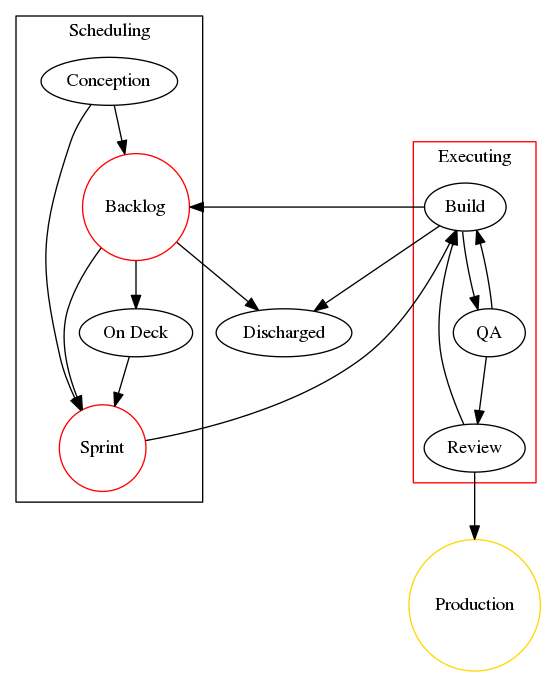
\includegraphics[width=15em]{workflow.png}
  \end{figure}

\end{frame}


\begin{frame}[fragile]
  \frametitle{Syntax and Semantics}

  \begin{figure}[p]
    \centering
    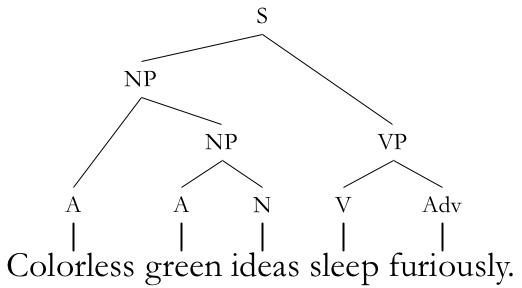
\includegraphics[width=15em]{sleep.png}
  \end{figure}

  \centering\huge{Don't Panic}\par

\end{frame}

\begin{frame}[fragile]
  \frametitle{Operators}

  Logical
  \begin{itemize}
  \item{AND}
  \item{OR}
  \item{NOT}
  \end{itemize}

  Conditional
  \begin{itemize}
  \item =
  \item !=
  \item \textasciitilde
  \item is
  \item is not
  \item in
  \item not in
  \end{itemize}

\end{frame}

\begin{frame}[fragile]
  \frametitle{Algebra all over again}

  \centering\huge{

  A AND B OR C

  A AND (B OR C)

  (A AND B) OR C

 }\par


\end{frame}

\begin{frame}[fragile]
  \frametitle{Fields and Values}
  
   \centering\large{

  project = Android OR project = iOS

  project in (Android, iOS) AND type = Bug

  (project != ATEAM) AND (text \textasciitilde \space Drawing)

 }\par

\end{frame}

\begin{frame}[fragile]
  \frametitle{Food and Questions Break}
   \begin{figure}[p]
    \centering
    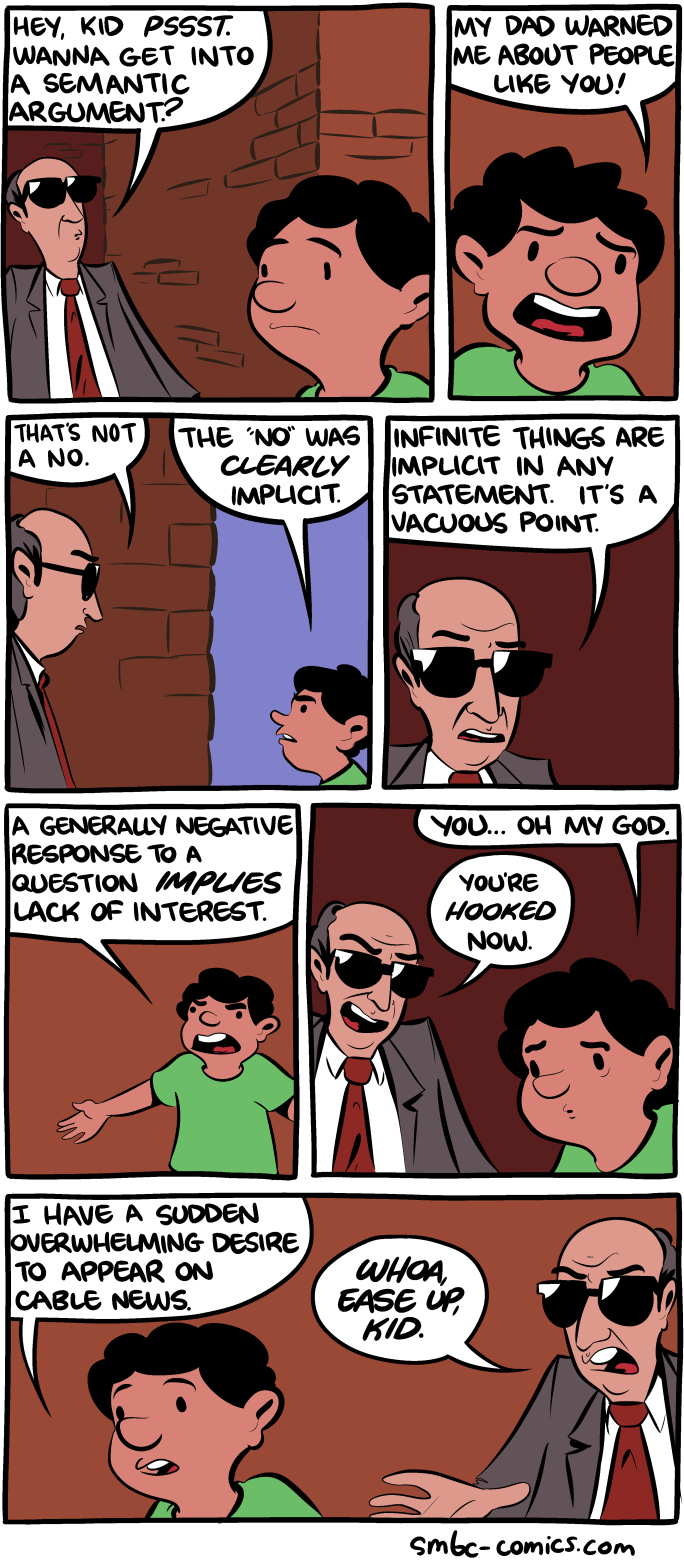
\includegraphics[width=15em]{comic.png}
  \end{figure}
\end{frame}
\begin{frame}[fragile]
  \frametitle{Integration and reuse}

  \begin{itemize}
  \item{Filters}
  \item{Boards}
  \item{Quick Filters}
  \item{Sharing}
  \item{Saving}
  \item{Webhooks!}
  \end{itemize}
  
\end{frame}

\begin{frame}[fragile]
  \frametitle{Gotchas}
  \begin{itemize}
  \item{Dates are goofy}
  \item{Editing a saved filter is dangerous}
  \item{Two types of sharing}
  \item{Different teams, different states}
  \item{Absolute truth and duplication}
  \end{itemize}
\end{frame}

\begin{frame}[fragile]
  \frametitle{Useful Queries}
  \centering\huge{\em This slide intentionally left blank}
\end{frame}

\end{document}
